\documentclass[oneside]{article}

\usepackage{blindtext} % Package to generate dummy text throughout this template 
\usepackage{graphicx} % FKM: for figures
\usepackage{wrapfig}
\usepackage{color} % FKM: for colored text
\usepackage{float} % FKM: for forcing figure placement
\usepackage[breakable]{tcolorbox} % FKM: for text box
\usepackage{enumerate} % FKM: for bullet point lists
\usepackage{setspace} % FKM: line spacing
\usepackage{soul} % strike through
\usepackage[normalem]{ulem} % strike through keeping emphasis standard
\usepackage{cancel} % diagonal strike through
\usepackage[margin=1in]{geometry} % FKM: margins

\usepackage[sc]{mathpazo} % Use the Palatino font
\usepackage[T1]{fontenc} % Use 8-bit encoding that has 256 glyphs
% \linespread{1.05} % Line spacing - Palatino needs more space between lines
\usepackage{microtype} % Slightly tweak font spacing for aestheticsgins
\usepackage[small,labelfont=bf,up,up]{caption} % Custom captions under/above floats in tables or figures
\usepackage{booktabs} % Horizontal rules in tables
\usepackage{amsmath} % Text in equations
\usepackage{titlesec} % Allows customization of titles
\usepackage{titling} % Customizing the title section
\usepackage[hidelinks]{hyperref} % For hyperlinks in the PDF

\usepackage{algorithm2e}

\usepackage{tikz}
\usetikzlibrary{shapes.geometric, arrows, positioning, decorations.markings, shapes.multipart}   
\usepackage{standalone}

\usepackage{subcaption} % for subfigures side by side
\captionsetup[subfigure]{singlelinecheck=false} % to put (a) and (b) at the top-left of subfigures

\usepackage[shortlabels]{enumitem} % customized lists (shortlabels
                                % necessary to have i., ii., etc., in enumerate)
\setlist[itemize]{noitemsep} % Make itemize lists more compact

\usepackage{abstract} % Allows abstract customization
\renewcommand{\abstractnamefont}{\normalfont\bfseries} % Set the "Abstract" text to bold
\renewcommand{\abstracttextfont}{\normalfont\small\itshape} % Set the abstract itself to small italic text

\usepackage{fancyhdr} % Headers and footers
\pagestyle{fancy} % All pages have headers and footers
\fancyhead{} % Blank out the default header
\fancyfoot{} % Blank out the default footer
\fancyhead[C]{Authors et al. $\bullet$ March 2022 $\bullet$ bio{\color{red}R}$\chi$ve} % Custom header text
\fancyfoot[RO,LE]{\thepage} % Custom footer text



\usepackage{natbib}
\bibliographystyle{apalike}

\usepackage{libertine}

\setlength\columnsep{20pt}

%----------------------------------------------------------------------------------------
%	TITLE SECTION
%----------------------------------------------------------------------------------------

\setlength{\droptitle}{-4\baselineskip} % Move the title up

%\pretitle{\begin{center}\Huge\bfseries} % Article title formatting
%\posttitle{\end{center}} % Article title closing formatting

\title{Validating Bayesian inference tools for phylogenetics} % Article title
%LM: strictly speaking, we're 'validating' the inference machinery.
%% Validating a model involves epistemic considerations that are, as far as I understand, outside the scope of this paper.
\author{\textsc{F\'{a}bio K. Mendes$^{1\dagger}$}, \textsc{Remco Bouckaert$^{2\dagger*}$},\\
\textsc{Luiz M. Carvalho$^{3\dagger}$}, \textsc{Alexei J. Drummond$^{4}$} \\
\small $^1$Department of Biology, Washington University in St. Louis\\
\small $^2$School of Computer Science, The University of Auckland\\
\small $^3$Escola de Matem\'{a}tica Aplicada, Fundaç\~{a}o Getulio Vargas\\
\small $^4$School of Biological Sciences, The University of Auckland\\
\small
\href{mailto:f.mendes@auckland.ac.nz}{$^*$Corresponding authors:
  f.mendes@auckland.ac.nz; remco@cs.auckland.ac.nz}\\
{\small $^\dagger$Authors contributed equally to this work}
% \href{mailto:f.mendes@auckland.ac.nz}{another.email@auckland.ac.nz}
%\and % Uncomment if 2 authors are required, duplicate these 4 lines if more
%\textsc{Jane Smith}\thanks{Corresponding author} \\[1ex] % Second author's name
%\normalsize University of Utah \\ % Second author's institution
%\normalsize \href{mailto:jane@smith.com}{jane@smith.com} % Second author's email address
}
\date{\today} % Leave empty to omit a date

\renewcommand{\figurename}{Supplementary Figure}
\renewcommand{\tablename}{Supplementary Table}

\doublespacing

\begin{document}

\maketitle

\begin{center}
    \Large Supplementary Material
\end{center}

\newpage
\section{Additional validation examples and guidelines}

\subsection{Validating a phylogenetic Brownian motion simulator}

In this section we focus on validating a simulator for the phylogenetic Brownian motion
model (``PhyloBM''; \citealp{felsenstein73}).
As explained in the main text, our goal is to verify that the expected value of certain
summary statistics (given a specific combination of parameter values) falls within its
$\alpha$-confidence intervals approximately $\alpha$\% of the time.
We will build confidence intervals about statistics calculated from several PhyloBM
samples of size \textcolor{red}{Z}, and then ask if the ``population'' value of 
a statistic -- given by the parameters of the multivariate normal sampling distribution --
is contained within its confidence interval frequently enough.

For summary statistics, we pay attention to the trait value's (i) species mean, (ii)
species variance, (iii) among-species covariance, and (iv) among-species correlation
coefficient.
Supplementary figure \ref{supfig:bmsimcis} shows one hundred confidence intervals for
each of these statistics, under multivariate normal $\text{MVN}(\boldsymbol{y},r\boldsymbol{T})$,
where $\boldsymbol{y}=\{0,0,0\}$, $r=0.1$ and $\boldsymbol{T}$ is given by the tree in
Fig. 2 in the main text.
Supplementary table \ref{suptab:bmsimcis} summarizes how often each statistic fell within
its 95\%-confidence interval.
These results indicate the PhyloBM simulator produces appropriate confidence intervals
and behaves as expected.

\begin{figure}
  \centering
  \includestandalone[width=14cm]{../figures/bmsim_cis}
  \caption{One hundred 95\%-confidence intervals (blue and red
    lines) built for summary statistics of interest.
    Red lines represent intervals that do not contain the value
    expected under the MVN sampling distribution characterizing
    the PhyloBM model.
    Parameter values are described in the text.}
  \label{supfig:bmsimcis}
\end{figure}

\begin{table}[h]
  \caption{The number of times $k$ that a summary
    statistic was contained within its corresponding
    95\%-confidence interval.
    Each statistic was calculated from 100 datasets of size
    \textcolor{red}{x} simulated
    under the PhyloBM model described in the text and in Box 1
    in the main text.}
  \label{suptab:bmsimcis}
  \centering
  \begin{tabular}{ c|c|c }
    \hline
    Statistic & Species $s$ (and $v$)& $k$\\
    \hline  
    $\text{E}[y_s]$ & A & 95\\
              & B & 97\\
              & C & 98\\
    $\text{Var}[y_s]$ & A & 93\\
              & B & 97\\
              & C & 97\\
    $\text{Cov}[y_s,y_v]$ & A and B & 95\\
              & A and C & 95\\
              & B and C & 97\\
    $\text{Cor}[y_s,y_v]$ & A and B & 96\\
              & A and C & 96\\
              & B and C & 97\\
    \hline
  \end{tabular}
\end{table}

\subsection{Validating a phylogenetic model with respect to a phylogenetic tree, $\Phi$}

Here, we expand on the discussion initiated in Box 2 in the main text.
We remind the reader that our goal is to validate the inference machinery
$\text{I}[\mathcal{M}]$ of a phylogenetic model $\mathcal{M}$, with
respect to one of its central parameters, phylogenetic tree $\Phi$.
More specifically, we would like to calculate the coverage probability of
$\Phi$ and to obtain its rank distribution.
Both tasks evaluate if $\mathcal{M}$ is well calibrated and correct.

Because of the nature of tree space, summarizing and comparing phylogenetic
trees with univariate measures is not a trivial task.
The key to an effective validation effort is to choose a functional
that reflects relevant estimators of the quantitiy of interest, in our case,
$\Phi$.
Fortunately, it is possible to exploit the metric nature of tree space and compute
quantities both from the generating phylogenetic tree $\Phi$ (i.e., the ``true''
tree sampled in the simulation stage of the validation process), as well as distances 
with respect to a reference phylogeny \st{$\tau_0$} $\Phi_0$.
We summarize some of these distances in supplementary table \ref{suptab:dists}.

\begin{table}[h]
  \caption{Phylogenetic space metrics (functionals) for investigating model correctness.}
  \label{suptab:dists}
  \centering
  \begin{tabular}{ c|c|c }
    \hline
    Metric & Notation & Ref. \\
    \hline  
    The largest branch length in $\Phi$ & $\text{LB}(\Phi)$ & N/A\\
    The length of $\Phi$ (the sum of all branch lengths & $\text{LEN}(\Phi)$ & N/A\\
    The length of the external branch leading to taxon $s_1$ & $\text{T}_1(\Phi)$ & N/A\\
    The Robinson-Foulds distance between $\Phi$ and $\Phi_0$ & $\text{RF}_0(\Phi)$ & \citep{Robinson1981}\\
    The Kendall-Coljin distance between $\Phi$ and $\Phi_0$ & $\text{KC}_0(\Phi;\omega)$ & \citep{Kendall2016}\\
    The Billera-Holmes-Vogtman distance between $\Phi$ and $\Phi_0$ & $\text{BHV}_0(\Phi)$ & \citep{Billera2001}\\
    \hline
  \end{tabular}
\end{table}

\textcolor{red}{[@Luiz: what is $\lambda$ in KC above? Previously,
     I have used $\lambda$ to represent the species birth-rate, as conventionally
     done with Yule models -- is there a better symbol here?]}
\textcolor{purple}{$\lambda \in (0, 1)$ is a weight that controls how much emphasis one wants to give to topological \textit{vs} branch lengths in the KC metric. I have changed it to $\omega$}.     
     

% \begin{itemize}
%  \item The largest branch length in \st{$\tau$} $\Phi$, \st{$M(\tau)$} $\text{LB}(\Phi)$;
%  \item The length of the phylogeny, i.e.,  the sum of branch lengths \st{$S(\tau)$} $\text{LEN}(\Phi)$;
%  \item The length of the external branch leading to taxon $s_1$, \st{$T_1(\tau)$} $\text{T}_1(\Phi)$;
%  \item The Robinson-Foulds \citep{Robinson1981} distance between \st{$\tau$} $\Phi$ and \st{$\tau_0$} $\Phi_0$, \st{$\operatorname{RF}_0(\tau)$} $\text{RF}_0(\Phi)$;
%  \item The Kendall-Coljin \citep{Kendall2016} distance between \st{$\tau$} $\Phi$ and \st{$\tau_0$} $\Phi_0$, \st{$\operatorname{KC}_0(\tau;\lambda)$} $\text{KC}_0(\Phi;\lambda)$; 
%  \item The Billera-Holmes-Vogtman (BHV) \citep{Billera2001} distance between \st{$\tau$} $\Phi$ and \st{$\tau_0$, $\operatorname{BHV}_0(\tau)$} $\Phi_0$, $\text{BHV}_0(\Phi)$;
% \end{itemize}

Once we have chosen a tree distance metric, we can now slightly modify
our SBC procedure and validate a model with respect to its
phylogenetic tree:
   
\RestyleAlgo{ruled}
\SetKwComment{Comment}{/* }{ */}

\begin{algorithm}[h]
  \DontPrintSemicolon
  \SetKwFunction{GenRefTree}{GenerateRefTree}
  \SetKwFunction{SampleTree}{SampleTree}
  \SetKwFunction{SampleData}{SampleData}
  \SetKwFunction{Distance}{CalculateDistance}
  \SetKwFunction{MCMC}{MCMC}
  \SetKwFunction{Rank}{GetRank}
  \caption{Algorithm for carrying out a simulation-based calibration procedure with respect to the phylogenetic tree parameter $\Phi$.}\label{alg:sbcphylo}
  $n \gets 100$\; \Comment*[r]{Number of data sets to simulate}
  $\phi_0 \gets$ \SampleTree{$\theta_\Phi$}\; \Comment*[r]{$\phi_0 \sim f(\Phi|\theta_\Phi)$}
  \For{$i \gets 1$ \KwTo $n$} {
    $\boldsymbol{\theta}_i \gets \text{S}[f(\theta)]$\; \Comment*[r]{$\boldsymbol{\theta_i} \sim f(\boldsymbol{\theta})$, with $\boldsymbol{\theta}_i = \{\theta_{i\Phi},\boldsymbol{\theta}_i^r\}$}
    $\phi_i \gets$ \SampleTree{$\theta_{i\Phi}$}\; \Comment*[r]{$\phi_i \sim f(\phi|\theta_{i\Phi})$}
    $d_i \gets$ \SampleData{$\phi_i,\boldsymbol{\theta}_i^r$}\; \Comment*[r]{$d_i \sim f(d|\phi_i,\boldsymbol{\theta}_i^r$}
    $\boldsymbol{\theta}_i^j \gets$ \MCMC{$f(\theta|d_i)$}\; \Comment*[r]{$\boldsymbol{\theta}_i = \{\boldsymbol{\theta}_i^j: j \in [1, L]\}$, where $L$ is the number of MCMC samples}
    $\bar{\delta}_i \gets$ \Distance{$\phi_0, \phi_i$}\; \Comment*[r]{According to a distance metric of choice}
    $\boldsymbol{\delta}_i^j \gets$ \Distance{$\phi_0, \phi_i^j$}\; \Comment*[r]{$\boldsymbol{\delta}_i = \{\delta_i^j: j \in [1, L]\}$}
    $r_i \gets$ \Rank($\bar{\delta}_i, \boldsymbol{\delta}_i^j$)\; \Comment*[r]{$r_i = \sum\limits_{j=1}^L \mathbb{I}(\delta^j_i < \bar{\delta_i})$}
  }
  \label{alg:sbc}
\end{algorithm}



  % \begin{enumerate}
  %   \setcounter{enumi}{-1}

  % \item Generate a reference tree from the prior $\bar{\tau}_0  \sim \pi_T(\tau | \boldsymbol \gamma)$; 

  %   \textbf{for} each iteration in 1:N, \textbf{do}:
    
  % \item Generate $\bar{\tau} \sim \pi_T(\tau | \boldsymbol \gamma)$;
  % \item Compute the distance $\bar{\delta} = d_\sigma(\bar{\tau},\bar{\tau}_0)$ according to the metric of choice;
  % \item Generate some (aligment) data $\tilde{y} \sim f(y | \bar{\tau}, \boldsymbol\alpha)$;
  % \item Draw (approximately) $\boldsymbol \tau_s = \{\tau_s^{(1)}, \tau_s^{(2)}, \ldots, \tau_s^{(L)}\}$ from the posterior $\pi(\tau | \tilde{y})$;
  % \item Compute distances $\boldsymbol \delta_s = \{ \delta_1, \delta_2, \ldots, \delta_L \}$  with $\delta_i = d_\sigma(\tau_s^{(i)}, \bar{\tau}_0)$;
  % \item Compute the rank $r(\boldsymbol\delta_s, \bar{\delta}) = \sum\limits_{i=1}^L \mathbb{I}(\delta_i < \bar{\delta})$.
  % \end{enumerate}

\begin{figure}
  \centering
  \vspace{0pt}
  \begin{subfigure}[t]{\textwidth}
    \caption{}
    \centering
    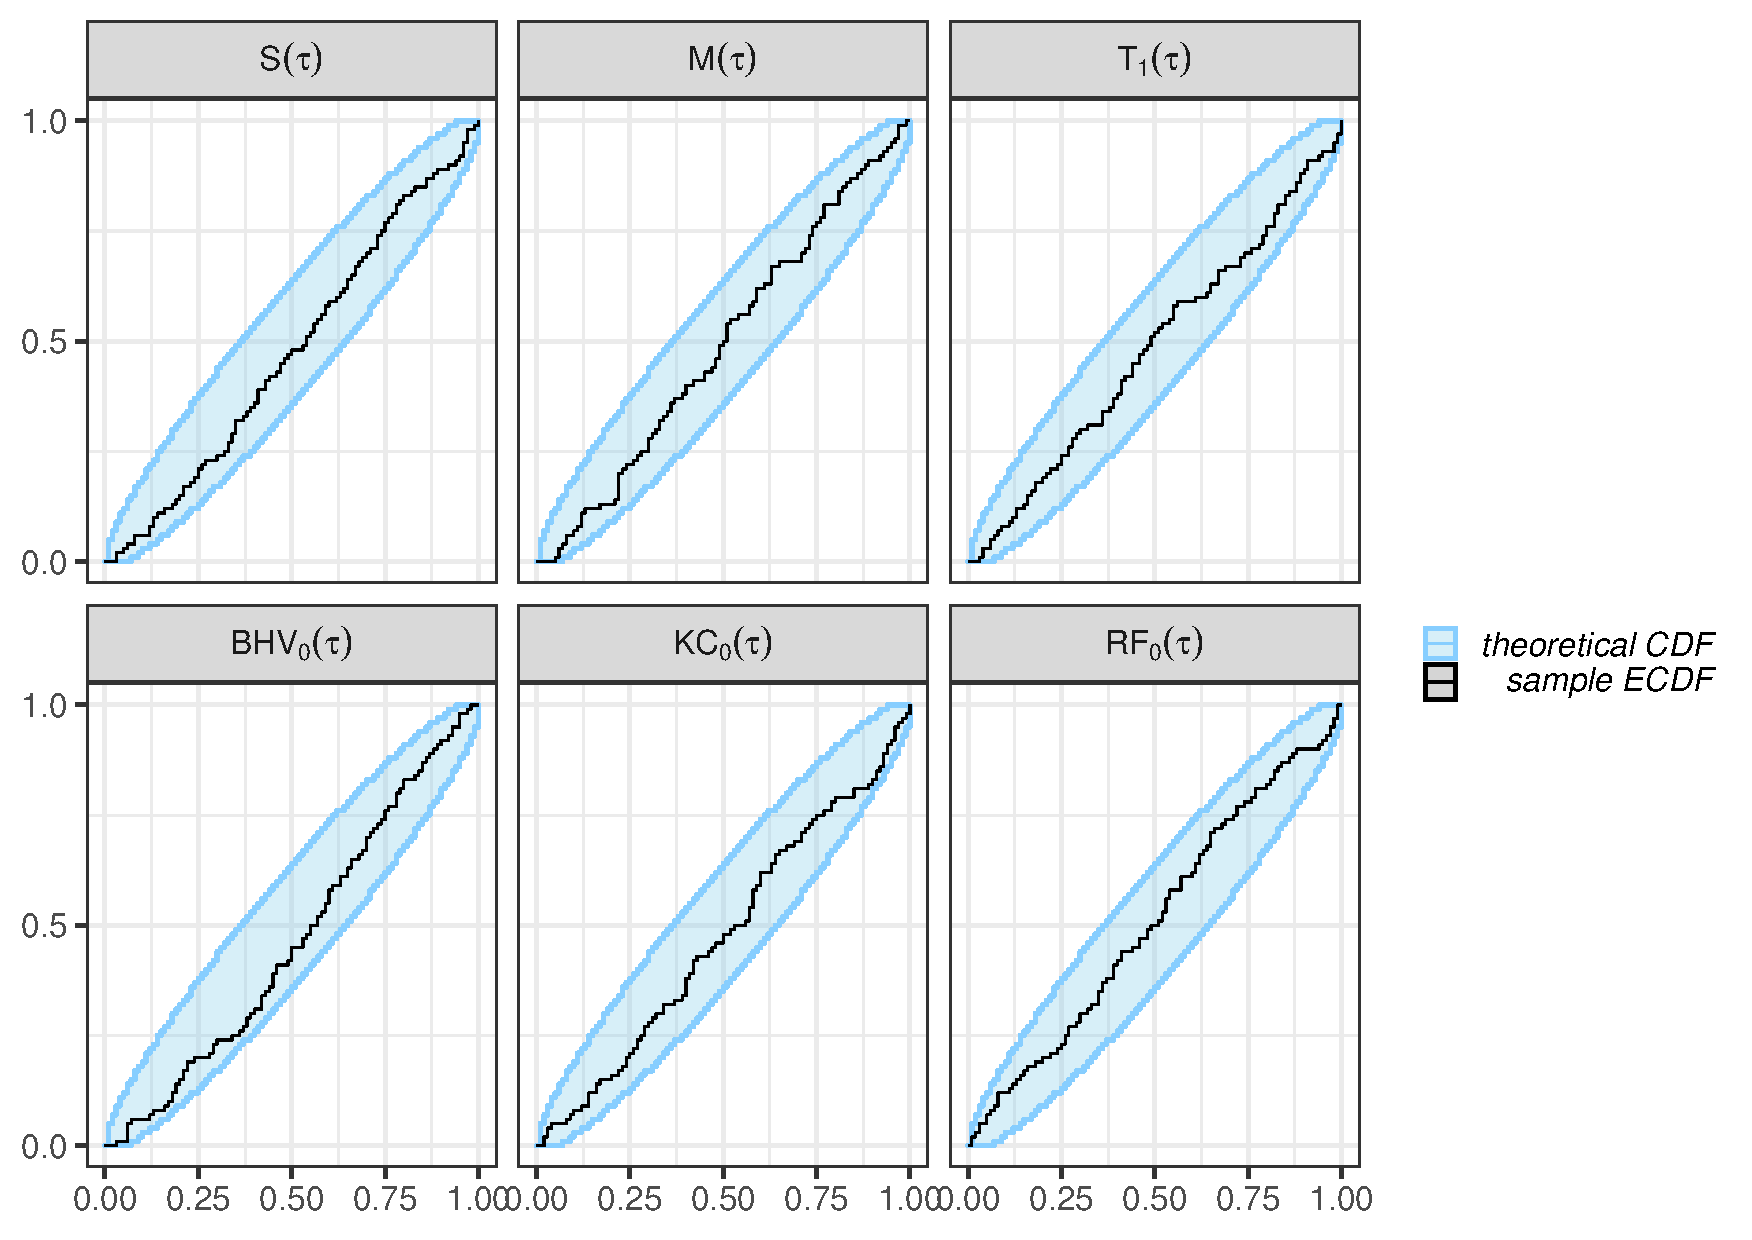
\includegraphics[scale=0.5]{../figures/ECDFs_SBC.pdf} 
  \end{subfigure}
  \vspace{0pt}
  \hspace{1cm}
  \begin{subfigure}[t]{\textwidth}
    \caption{}
    \centering
    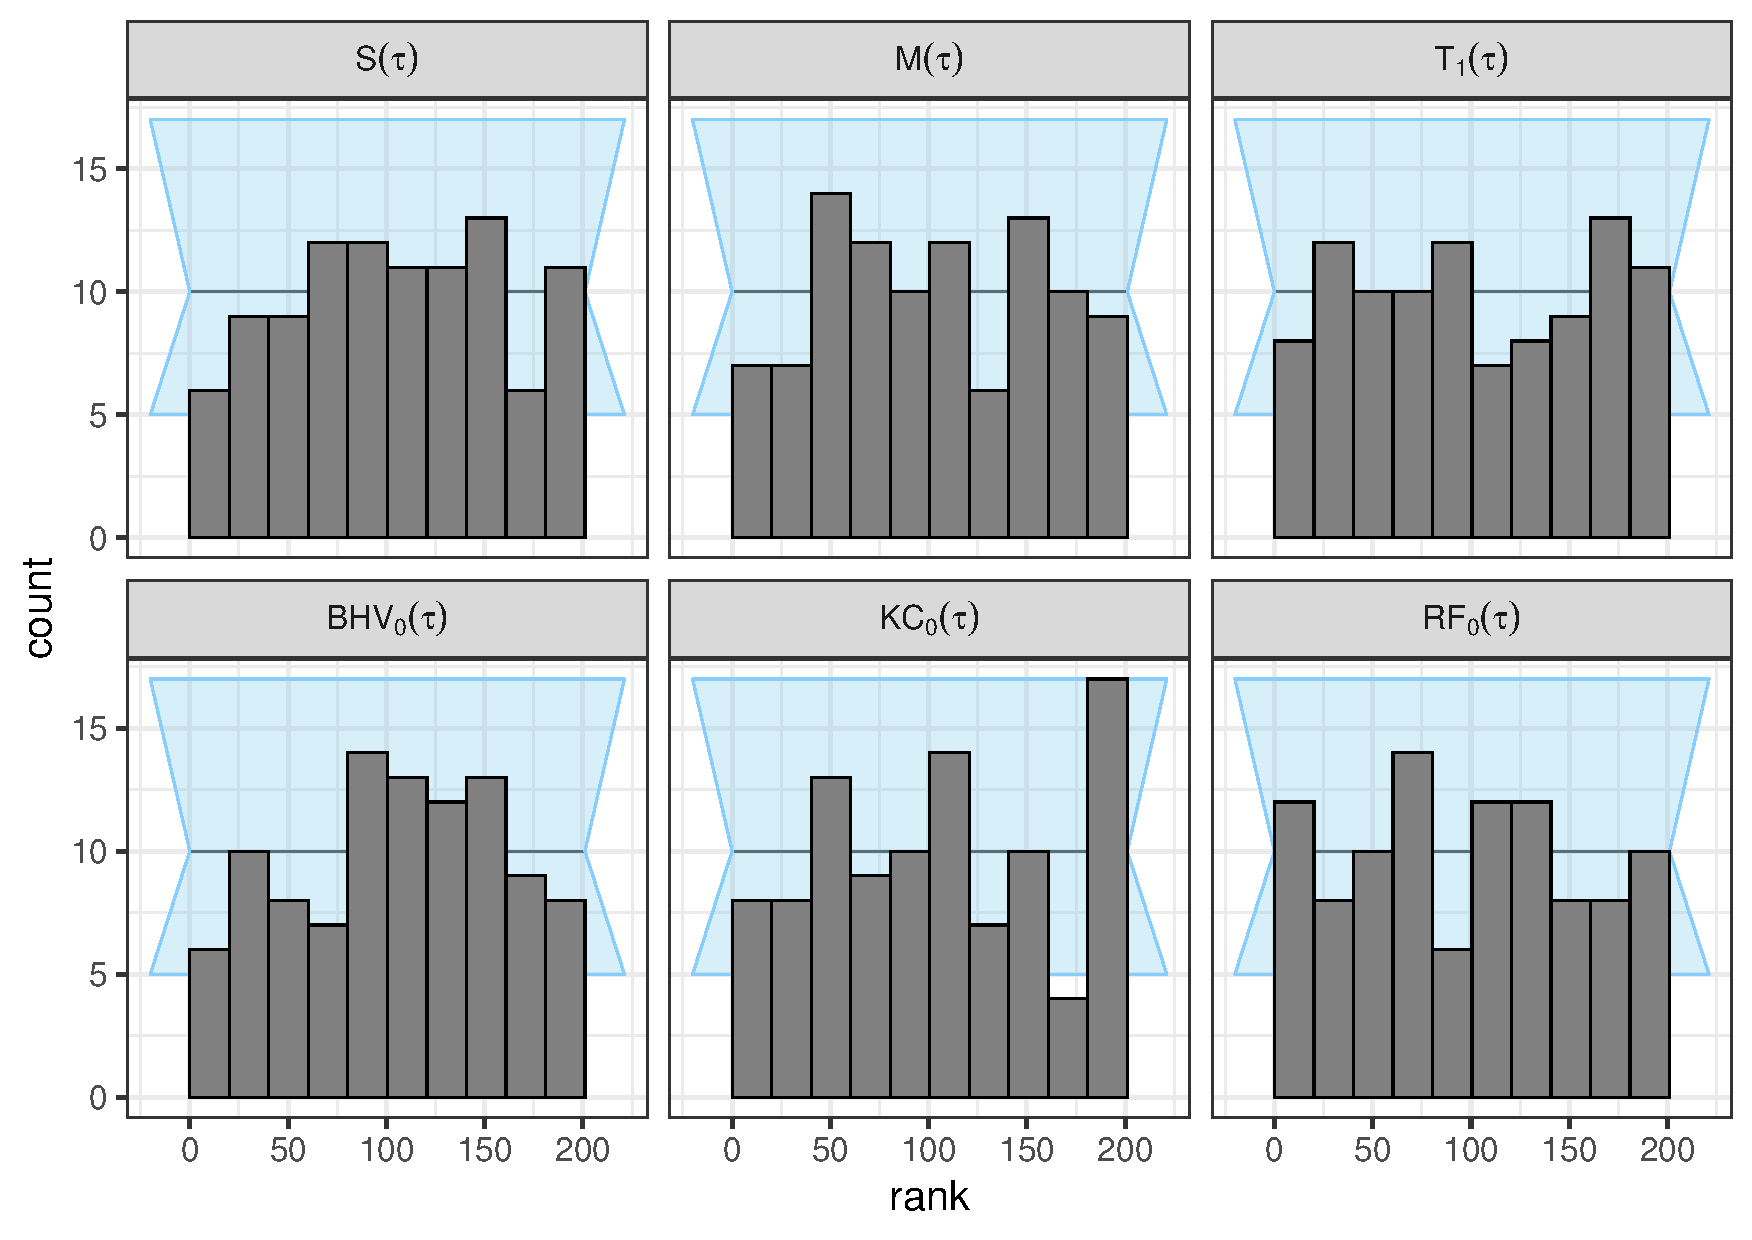
\includegraphics[scale=0.5]{../figures/hists_SBC.pdf}    
  \end{subfigure}
  \hfill
   \caption{Simulation-based calibration (SBC) of a phylogenetic
     model, focusing on the phylogenetic tree parameter.
     (a) Empirical cumulative distribution function (ECDF) for each
     functional.
     (b) Rank distribution for each functional.
   \textcolor{red}{[@Luiz: Need to fix notation in this figure,
     replacing $\tau$ with $\Phi$; I changed the abbreviation of some
     of the functionals as well, to avoid collision (see the table
     above);
     the x-axis labels in panel(a)
     are also overlapping each other]; ``rank'' and ``count''
     should start with uppercase ``Rank'', ``Count''}}
   \label{supfig:sbc}
\end{figure}

\begin{figure}
 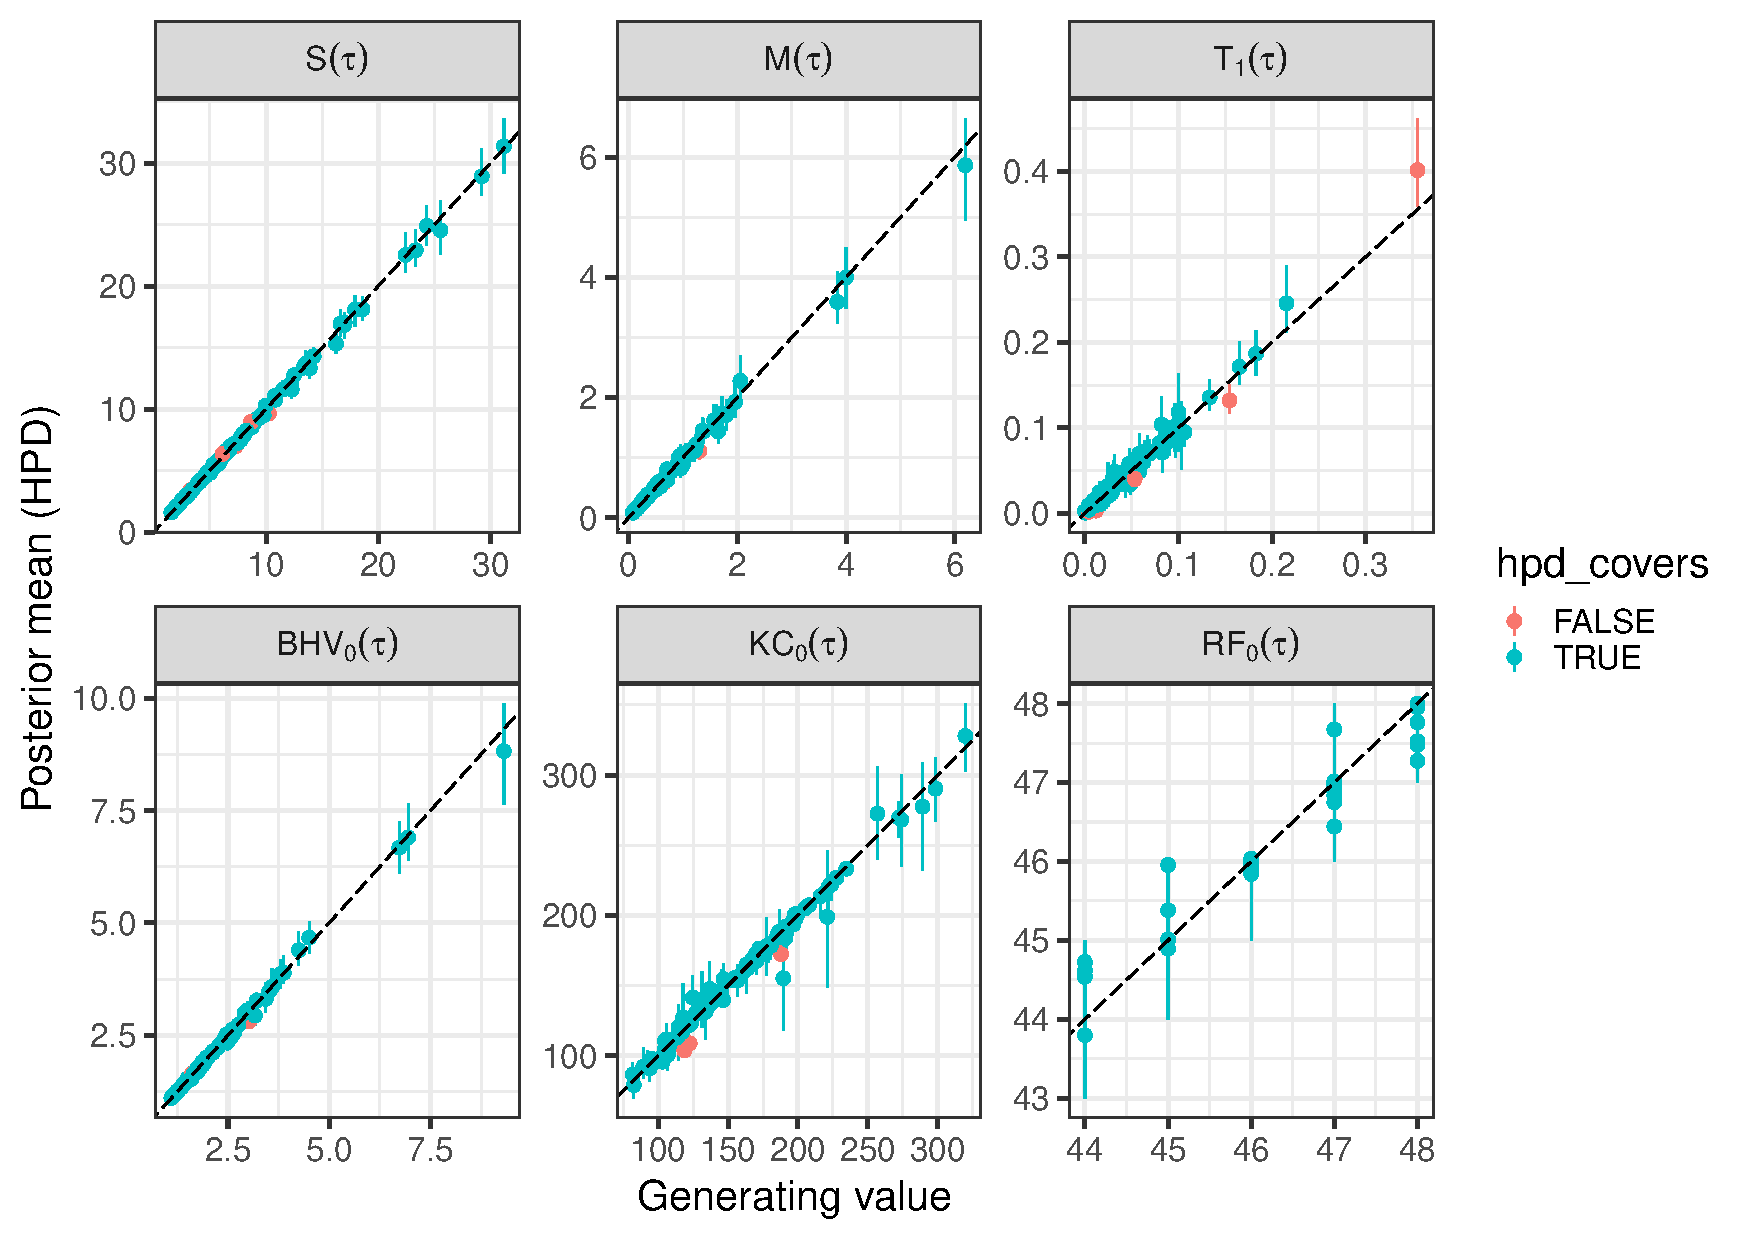
\includegraphics[width=\textwidth]{../figures/coverage.pdf}
    \caption{Coverage for different functionals in validation experiment
      \textcolor{red}{[@Luiz: maybe we can use
        ``SBC'' to refer just to the experiment looking at ECDFs and
        ranks -- see main text; also I would
     remove the legend entirely and keep just the description
   in the caption]}
        % simulation-based calibration.
      Posterior means are represented by point and 95\% HPDs by bars.
      Red dots and lines show intervals that failed to include the
      generating value, whilst blue ones show those that did include
      the simulated ``truth''.}
  \label{supfig:phylo_calibration}
\end{figure}

Supplementary figure \ref{supfig:sbc} summarizes the results for the functionals
listed in table \ref{suptab:dists}.
As can be seen, the ECDFs lie well inside their confidence ellipses
and the observed ranks also lie inside their confidence bands.

Finally, we can also investigate if our model is well-calibrated
by examining the coverage probability of 95\%-HPDs over the chosen
tree metrics.
Supplementary figure \ref{supfig:phylo_calibration} shows that the HPDs do cover the
generating metrics with probability compatible with what is expected
theoretically.
% In this instance, the tests would fail to detect problems with the algorithm.
% These plots can be supplemented with a table showing attained coverage and binomial confidence intervals for this quantity (see Table~\ref{tab:coverage}).
% A further advantage of graphically investigating coverage is that one can identify consistent areas for which estimation fails -- e.g. high/low simulated values of a given variable.

\newpage
\section{Proof for coverage validation}
% \label{appendix::sec:proofs}

For a number $n$ of simulations, simulate

\begin{align*}
\theta^{(i)} &\sim f(\cdot), \\
y^{(i)} \mid \theta^{(i)} &\sim f(\cdot \mid \theta^{(i)}).
\end{align*}

Now  for brevity, define $a^{(i)} := a(y^{(i)}, \alpha)$ and $b^{(i)} := b(y^{(i)}, \alpha)$ and recall $I_{\alpha}\left(y^{(i)}\right)$ is such that 

\begin{align*}
Q\left(b^{(i)} \mid y^{(i)}\right) - Q\left(a^{(i)} \mid y^{(i)}\right) = p_1 - p_2 = \alpha,
\end{align*}

\noindent where $Q_{y}(x)$ is the posterior (conditional on data $y$) CDF and $p_1, p_2 \in (0,1)$, with $p_1 < p_2$.
A natural quantity to compute is:

\begin{align*}
S_n = n^{-1}\sum_{i=1}^n \mathbb{I}\left(\theta^{(i)} \in I_{\alpha}\left(y^{(i)}\right) \right),
\end{align*}

\noindent i.e., the attained coverage of the Bayesian intervals.
Let $F_U(x) = x$ be the CDF of a $\operatorname{Uniform(0, 1)}$ random variable. 
Now we can consider what happens when the number of simulations grows, i.e., the limit $\lim_{n \to \infty} S_n$.
We may re-write the limit as:

\begin{align*}
\lim_{n \to \infty} S_n &= \lim_{n \to \infty} n^{-1}\sum_{i=1}^n \mathbb{I}\left(\theta^{(i)} \in I_{\alpha}\left(y^{(i)}\right) \right),\\
&=  \lim_{n \to \infty} n^{-1}\sum_{i=1}^n \left\{ \mathbb{I}\left(\theta^{(i)} \leq b^{(i)} \right) - \mathbb{I}\left(\theta^{(i)} \leq a^{(i)} \right) \right\},\\
&=  \lim_{n \to \infty} n^{-1}\sum_{i=1}^n \mathbb{I}\left(\theta^{(i)} \leq b^{(i)} \right) -  n^{-1}\sum_{i=1}^n\mathbb{I}\left(\theta^{(i)} \leq a^{(i)} \right),\\
&=  \lim_{n \to \infty} n^{-1}\sum_{i=1}^n \mathbb{I}\left(Q_{y^{(i)}}^{-1}\left(\theta^{(i)}\right) \leq p_1 \right) -   \lim_{n \to \infty} n^{-1}\sum_{i=1}^n\mathbb{I}\left(Q_{y^{(i)}}^{-1}\left(\theta^{(i)}\right) \leq p_2 \right),\\
&= F_U(p_1) - F_U(p_2) = \alpha,
\end{align*}

\noindent where the last line follows from the fact that the CDF of $\theta^{(i)}$ is uniformly distributed on $(0, 1$) (Theorem 1 in \cite{Cook2006}) and almost sure convergence of the ECDF to the true CDF due to the  Glivenko-Cantelli theorem~\cite[page 275]{Billingsley1986}.
\bibliography{refs}

\end{document}
